% Final presentation — pdflatex Final_Presentation.tex (run twice for TOC)
% Figures: presentation_figures/*.png (from notebooks + python extract_notebook_figures.py)
\documentclass[aspectratio=169, 11pt]{beamer}

\usepackage{tikz}
\usetikzlibrary{shapes.geometric, arrows.meta, positioning, calc, fit, backgrounds, decorations.pathreplacing}
\usepackage{amsmath, amssymb}
\usepackage{booktabs}
\usepackage{graphicx}
\usepackage{xcolor}
\usepackage{fontawesome5}
\usepackage{multirow}
\usepackage{array}
\usepackage{adjustbox}

\usetheme{Madrid}
\usecolortheme{seahorse}

\definecolor{vflblue}{RGB}{41, 128, 185}
\definecolor{vflgreen}{RGB}{39, 174, 96}
\definecolor{vflred}{RGB}{231, 76, 60}
\definecolor{vflorange}{RGB}{243, 156, 18}
\definecolor{vflpurple}{RGB}{142, 68, 173}
\definecolor{vflgray}{RGB}{127, 140, 141}
\definecolor{lightbg}{RGB}{248, 249, 250}
\definecolor{deepblue}{RGB}{0, 51, 102}

\setbeamercolor{frametitle}{bg=vflblue, fg=white}
\setbeamercolor{title}{fg=vflblue}
\setbeamercolor{block title}{bg=vflblue, fg=white}
\setbeamercolor{block body}{bg=lightbg}
\setbeamercolor{block title alerted}{bg=vflred, fg=white}
\setbeamercolor{block title example}{bg=vflgreen, fg=white}

\setbeamertemplate{navigation symbols}{}
\setbeamertemplate{footline}[frame number]

\graphicspath{{./presentation_figures/}{./Part4_figures/}{./presentation_figures_vfu_verification/}{./}}

% Include slide PNG if present; otherwise show a small boxed note (no broken compile).
\newcommand{\SlideFig}[2]{%
  % Robust include: keep aspect ratio and constrain height so it always fits the slide.
  \IfFileExists{#1}{%
    \includegraphics[width=#2,height=0.72\textheight,keepaspectratio]{#1}%
  }{%
    \IfFileExists{presentation_figures/#1}{%
      \includegraphics[width=#2,height=0.72\textheight,keepaspectratio]{presentation_figures/#1}%
    }{%
      \IfFileExists{Part4_figures/#1}{%
        \includegraphics[width=#2,height=0.72\textheight,keepaspectratio]{Part4_figures/#1}%
      }{%
        \begin{center}
        \fbox{\parbox{0.86\linewidth}{\centering\vspace{0.9em}\small
        \textbf{Missing figure:} \texttt{#1}\\[0.35em]
        Expected in \texttt{presentation\_figures/} or \texttt{Part4\_figures/}.\\
        Re-run the notebook cells that generate the plots.\vspace{0.9em}}}
        \end{center}%
      }%
    }%
  }%
}

\title[E-VFU]{E-VFU: Multi-Attack Verification for Vertical Federated Unlearning}
\subtitle{PETS-style \textsc{VFU-KD} / \textsc{VFU-GA} with extended verification and feature-entanglement discussion}
\author{Gourab Biswas \and Fairuz}
\institute{Undergraduate machine learning project}
\date{\today}

\begin{document}

\begin{frame}
  \titlepage
\end{frame}

\begin{frame}{Outline}
  \tableofcontents
\end{frame}

% =============================================================================
\section{Introduction: problem \& motivation}
% =============================================================================

\begin{frame}{Vertical Federated Learning (VFL)}
  \begin{columns}[T]
    \begin{column}{0.52\textwidth}
      \begin{block}{\faArrowsAltH\ Horizontal FL}
        \textbf{Same features, different samples} (e.g., many hospitals, same tests, different patients).
      \end{block}
      \vspace{0.35em}
      \begin{exampleblock}{\faArrowsAltV\ Vertical FL}
        \textbf{Same samples, different features} (e.g., bank + hospital + label holder for the same user IDs).
      \end{exampleblock}
      \vspace{0.35em}
      Parties exchange \textbf{embeddings} or gradients --- not raw joint feature vectors.
    \end{column}
    \begin{column}{0.44\textwidth}
      \begin{center}
      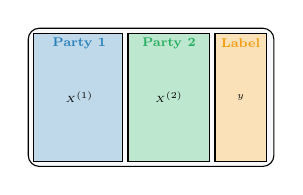
\begin{tikzpicture}[scale=0.65, transform shape]
        \draw[fill=lightbg, rounded corners] (-2.4,-1.35) rectangle (2.4,1.35);
        \draw[fill=vflblue!30] (-2.3,-1.25) rectangle (-0.55,1.25);
        \node[font=\scriptsize\bfseries, vflblue] at (-1.4,1.05) {Party 1};
        \draw[fill=vflgreen!30] (-0.45,-1.25) rectangle (1.15,1.25);
        \node[font=\scriptsize\bfseries, vflgreen] at (0.35,1.05) {Party 2};
        \draw[fill=vflorange!30] (1.25,-1.25) rectangle (2.25,1.25);
        \node[font=\scriptsize\bfseries, vflorange] at (1.75,1.05) {Label};
        \node[font=\tiny] at (-1.4,0) {$X^{(1)}$};
        \node[font=\tiny] at (0.35,0) {$X^{(2)}$};
        \node[font=\tiny] at (1.75,0) {$y$};
      \end{tikzpicture}
      \end{center}
    \end{column}
  \end{columns}
\end{frame}

\begin{frame}{Why unlearning in VFL?}
  \begin{enumerate}
    \item \textbf{Right to erasure} (GDPR): data must be removed from trained models, not only from databases.
    \item Unlearning targets: \textbf{client} (party leaves), \textbf{feature} (column forgotten), or \textbf{sample} (specific rows).
    \item Full retraining is costly $\Rightarrow$ approximate methods (\textsc{VFU-KD}, \textsc{VFU-GA}, fine-tuning).
  \end{enumerate}
  \vspace{0.4em}
  \begin{alertblock}{Core question}
    \textbf{How do we \emph{verify} that unlearning worked?} Weak metrics can declare success while stronger attacks still detect membership or artifacts.
  \end{alertblock}
\end{frame}

\begin{frame}{Base paper: Varshney et al.\ (PETS 2025)}
  \begin{itemize}
    \item Feature-level VFL unlearning: \textbf{VFU-KD} (distillation) and \textbf{VFU-GA} (gradient ascent).
    \item Active party may retrain a student / run ascent; passive encoders may stay frozen.
    \item Evaluation includes \textbf{output-based} membership inference (MIA).
  \end{itemize}
  \vspace{0.35em}
  \begin{alertblock}{Why go beyond output MIA?}
    Logits are not the whole story: gradients and internal representations can still leak membership. Stronger MIAs are a stricter test of whether unlearning actually held.
  \end{alertblock}
\end{frame}

\begin{frame}{What we add on top of PETS}
  \begin{enumerate}
    \item \textbf{Gradient MIA} and \textbf{shadow-model} meta-classification alongside output MIA.
    \item \textbf{Feature entanglement:} correlated columns across parties mean party $k$'s signal may partly live in party $j$'s encoder; we discuss cross-party Jacobian-style diagnostics (see also LASER-VFL on missing features).
    \item \textbf{Open engineering questions:} secure-aggregation cost, repeated unlearning rounds.
  \end{enumerate}
  \vspace{0.4em}
  \textbf{E-VFU:} keep PETS-style unlearning; add \textbf{four verification attacks} with clear pass/fail-style targets.
\end{frame}

% =============================================================================
\section{Dataset and statistics}
% =============================================================================

\begin{frame}{Datasets and VFL split (statistics)}
  \begin{center}
  \small
  \begin{tabular}{@{}lrrp{4.6cm}@{}}
    \toprule
    \textbf{Dataset} & \textbf{Samples} & \textbf{Features} & \textbf{Target / balance} \\
    \midrule
    UCI Adult & 30{,}162 & 14 & Income $>$50K: 7{,}508 vs.\ 22{,}654 ($\sim$25\% positive) \\
    German Credit & 1{,}000 & 20 & Good vs.\ bad: 700 / 300 \\
    Bank Marketing & 41{,}188 & 16 & Term deposit: imbalanced (minority positive) \\
    Credit Card Default & 30{,}000 & 23 & Default: imbalanced (minority positive) \\
    \bottomrule
  \end{tabular}
  \end{center}
  \vspace{0.45em}
  \begin{itemize}
    \item Label encoding for categoricals; drop Adult rows with missing values; \textbf{per-party standardization}.
    \item Features partitioned across \textbf{2--3 parties}; one active party holds \textbf{labels}.
    \item Stratified train/val/test, seed 42.
  \end{itemize}
\end{frame}

% =============================================================================
\section{Architecture and training}
% =============================================================================

\begin{frame}{Model architecture (Phase 0)}
  \begin{columns}[T]
    \begin{column}{0.32\textwidth}
      \begin{block}{\faLayerGroup\ Bottom encoders}
        \footnotesize
        Each passive party: MLP on local $X^{(k)} \to$ embedding $e_k$.
      \end{block}
    \end{column}
    \begin{column}{0.32\textwidth}
      \begin{exampleblock}{\faSitemap\ Top model}
        \footnotesize
        $[e_1 \| \cdots \| e_K] \to$ MLP $\to$ sigmoid; \textbf{BCE} during training.
      \end{exampleblock}
    \end{column}
    \begin{column}{0.32\textwidth}
      \begin{alertblock}{\faCogs\ Unlearning}
        \footnotesize
        \textsc{VFU-KD}: student top / student bottom + teacher.\\
        \textsc{VFU-GA}: ascent on target subset.
      \end{alertblock}
    \end{column}
  \end{columns}
  \vspace{0.4em}
  \begin{center}
    \footnotesize
    \colorbox{yellow!25}{\textbf{Training (typical):} Adam or RAdam, lr $\approx 10^{-3}$, on the order of tens of epochs, batch 256--512.}
  \end{center}
\end{frame}

% =============================================================================
\section{Loss functions and intuition}
% =============================================================================

\begin{frame}{VFU-GA: intuition}
  \begin{columns}[T]
    \begin{column}{0.55\textwidth}
      Training: $\theta \leftarrow \theta - \eta \nabla \mathcal{L}$.\quad
      Unlearning: $\theta \leftarrow \theta \textcolor{vflred}{\mathbf{+}} \eta \nabla \mathcal{L}$ on \textbf{target} samples.
      \vspace{0.5em}
      \begin{itemize}
        \item Fast; implement by negating the task loss on the forget set.
        \item Risk: utility drop; may leave \textbf{forensic} traces (FUMA-sensitive).
      \end{itemize}
    \end{column}
    \begin{column}{0.42\textwidth}
      \begin{center}
      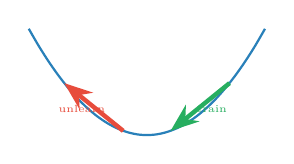
\begin{tikzpicture}[scale=0.75, transform shape]
        \draw[thick, domain=-2:2, smooth, variable=\x, vflblue] plot ({\x}, {0.45*\x*\x});
        \draw[-{Stealth}, ultra thick, vflgreen] (1.4, 0.88) -- (0.4, 0.07);
        \draw[-{Stealth}, ultra thick, vflred] (-0.4, 0.07) -- (-1.4, 0.88);
        \node[font=\tiny, vflgreen] at (1.1, 0.45) {train};
        \node[font=\tiny, vflred] at (-1.1, 0.45) {unlearn};
      \end{tikzpicture}
      \end{center}
    \end{column}
  \end{columns}
\end{frame}

\begin{frame}{VFU-KD: loss}
  \begin{center}
  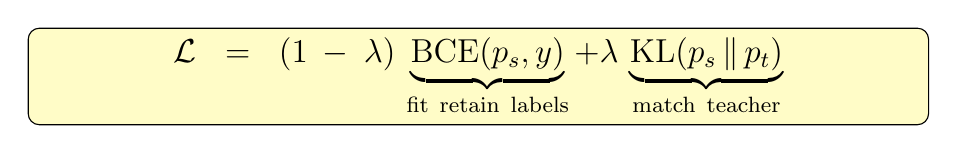
\begin{tikzpicture}
    \node[draw, rounded corners, fill=yellow!22, text width=11.2cm, align=center, font=\large] {
      $\mathcal{L} = (1-\lambda)\,\underbrace{\mathrm{BCE}(p_s, y)}_{\text{fit retain labels}}
      + \lambda\,\underbrace{\mathrm{KL}(p_s \,\|\, p_t)}_{\text{match teacher}}$
    };
  \end{tikzpicture}
  \end{center}
  \vspace{0.35em}
  \begin{itemize}
    \item Student sees embeddings \textbf{without} removed party (or reduced features); teacher is \textbf{frozen} pre-unlearning model.
    \item \textbf{Intuition:} BCE keeps task accuracy on retain data; KL preserves decision boundary \emph{as if} the old fusion still had access, while dropping the forgotten party from the forward pass.
    \item In our code, $\lambda = 0.3$ is a typical distillation weight; other runs use temperature-scaled KL with a different $\alpha$ (same trade-off, different parameterization).
  \end{itemize}
\end{frame}

\begin{frame}{Unlearning methods at a glance}
  \begin{center}
  \small
  \begin{tabular}{lccc}
    \toprule
    \textbf{Aspect} & \textbf{VFU-GA} & \textbf{VFU-FT} & \textbf{VFU-KD} \\
    \midrule
    Speed & fast & medium & slower \\
    Utility & can drop & good & best (typ.) \\
    Forgetting & strong & medium & strong \\
    \bottomrule
  \end{tabular}
  \end{center}
  \vspace{0.5em}
  \begin{alertblock}{\faLightbulb\ Recommendation}
    Use \textsc{VFU-GA} for quick removal when utility loss is OK; use \textsc{VFU-KD} when quality matters. \textbf{Always} run multi-attack verification afterward.
  \end{alertblock}
\end{frame}

% =============================================================================
\section{Feature entanglement perspective}
% =============================================================================

\begin{frame}{Feature entanglement: why it matters for VFU}
  \begin{itemize}
    \item Shared loss couples all encoders; \textbf{correlated} columns across parties let $f_j$ exploit patterns that partly ``stand in'' for removed party $k$.
    \item Removing $X_k$ can cause \textbf{collateral} drops for remaining parties (reported $>$18\% in some missing-feature studies, e.g.\ LASER-VFL narrative).
  \end{itemize}
  \vspace{0.35em}
  \begin{block}{Jacobian-based diagnostic (optional extension)}
    Measure cross-party sensitivity, e.g.\ $J^{(l)}_{k\to j} = \partial h_j^{(l)} / \partial X_k$, and summarize the spectrum (SVD) to flag high influence \emph{before} unlearning. This complements black-box MIA checks.
  \end{block}
\end{frame}

\begin{frame}{Where Jacobian + cross-party + VFL meet}
  \begin{center}
  \footnotesize
  \renewcommand{\arraystretch}{1.2}
  \begin{tabular}{lccc}
    \toprule
    & \textbf{Jacobian tool} & \textbf{Cross-party} & \textbf{VFL unlearning} \\
    \midrule
    Same-party Jacobian defences (e.g.\ SensFL) & \checkmark & --- & partial \\
    Certified VFU / constraint methods & --- & \checkmark & \checkmark \\
    \textbf{This project} & \checkmark & \checkmark & \checkmark \\
    \bottomrule
  \end{tabular}
  \end{center}
  \vspace{0.4em}
  Verification attacks ask whether the model still \emph{remembers}; entanglement analysis asks how tightly parties were coupled before anyone left.
\end{frame}

% =============================================================================
\section{Related work and SOTA positioning}
% =============================================================================

\begin{frame}{Comparison with selected prior work}
  \begin{center}
  \scriptsize
  \begin{tabular}{@{}p{2.5cm}p{3.8cm}p{4.8cm}@{}}
    \toprule
    \textbf{Line} & \textbf{Representative} & \textbf{vs.\ our project} \\
    \midrule
    HFL unlearning & FedEraser, SISA, KNOT & Different partition (rows vs.\ columns). \\
    VFL unlearning & VFU-LR; Gu et al.\ few-shot & Other mechanisms; we build on PETS \textsc{VFU-KD/GA}. \\
    PETS 2025 & Varshney et al. & Unlearning algorithms we implement. \\
    This project & E-VFU + Jacobian angle & Heavier \textbf{verification stack}; optional entanglement discussion. \\
    \bottomrule
  \end{tabular}
  \end{center}
\end{frame}

% =============================================================================
\section{E-VFU verification framework}
% =============================================================================

\begin{frame}{E-VFU in one slide}
  \begin{block}{Phase 0}
    Train VFL model; run \textsc{VFU-KD} and/or \textsc{VFU-GA} as in PETS-style setup.
  \end{block}
  \begin{block}{Phase 1 --- four auditors}
    \begin{enumerate}
      \item \textbf{Output MIA} (Varshney baseline): target AUC $\approx 0.5$ on unlearned samples.
      \item \textbf{Gradient MIA}: norms + layer stats + spectral features $\Rightarrow$ Random Forest.
      \item \textbf{FUMA}: forensic before/after detector on (prediction, loss, gradient-change) features; target low detectability.
      \item \textbf{Shadow models}: model-level meta-classifier --- does unlearned model look ``retain-only''?
    \end{enumerate}
  \end{block}
\end{frame}

\begin{frame}{What we intended vs.\ what we observed (rubric-friendly)}
  \begin{block}{Intent (verification goal)}
    After unlearning, the model should be \textbf{useful} on test data but \textbf{indistinguishable} from a model that never saw the target data.
  \end{block}
  \vspace{0.35em}
  \begin{columns}[T]
    \begin{column}{0.49\textwidth}
      \begin{exampleblock}{What we implemented}
        \begin{itemize}
          \item PETS-style \textsc{VFU-GA} and \textsc{VFU-KD} (plus FT baseline).
          \item Multi-attack auditing: Output-MIA, Gradient-MIA, FUMA, Shadow.
          \item Cross-dataset experiments (Adult, German, Bank, Credit Card).
        \end{itemize}
      \end{exampleblock}
    \end{column}
    \begin{column}{0.49\textwidth}
      \begin{alertblock}{What we observed}
        \begin{itemize}
          \item Utility often stays high, but \textbf{verification signals can disagree}.
          \item Gradient/forensic/model-level attacks can reveal traces even when logits-based MIA is near chance.
          \item Stronger auditing reduces false ``pass'' conclusions.
        \end{itemize}
      \end{alertblock}
    \end{column}
  \end{columns}
\end{frame}

\begin{frame}{Why four attacks?}
  \begin{center}
  \begin{tikzpicture}[scale=0.88, transform shape]
    \node[draw, rounded corners, fill=vflblue!28, minimum width=2.7cm, minimum height=1.05cm, align=center, font=\scriptsize] at (-4.8, 0) {\faSearch\\Output MIA};
    \node[draw, rounded corners, fill=vflgreen!28, minimum width=2.7cm, minimum height=1.05cm, align=center, font=\scriptsize] at (-1.6, 0) {\faWaveSquare\\Gradient MIA};
    \node[draw, rounded corners, fill=vflorange!28, minimum width=2.7cm, minimum height=1.05cm, align=center, font=\scriptsize] at (1.6, 0) {\faFingerprint\\FUMA};
    \node[draw, rounded corners, fill=vflpurple!28, minimum width=2.7cm, minimum height=1.05cm, align=center, font=\scriptsize] at (4.8, 0) {\faClone\\Shadow};
  \end{tikzpicture}
  \end{center}
  \vspace{0.35em}
  Covers \emph{outputs}, \emph{gradients}, \emph{probe behavior}, and \emph{global model fingerprint}. Passing only (1) does not imply passing (2)--(4).
\end{frame}

\begin{frame}{Success criteria (summary)}
  \begin{center}
  \footnotesize
  \begin{tabular}{@{}p{2.9cm}p{3.0cm}p{4.5cm}@{}}
    \toprule
    \textbf{Component} & \textbf{Metric} & \textbf{Desirable outcome} \\
    \midrule
    Output MIA & AUC & $\approx 0.5$ \\
    Gradient MIA & AUC / $\Delta\|g\|$ & near chance + large shift on targets \\
    FUMA & Detection rate & low (e.g.\ $<5\%$) \\
    Shadow & P(full data) & $< 0.5$ for unlearned model \\
    \bottomrule
  \end{tabular}
  \end{center}
\end{frame}

% =============================================================================
\section{Experiments and results}
% =============================================================================

\begin{frame}{Experimental setup}
  \begin{itemize}
    \item 4 public tabular datasets; VFL simulated by splitting feature columns across parties; binary classification.
    \item \textbf{Forget set:} typically 5\% of training indices (sample unlearning in Part~4), or a removed party / column group (feature/client unlearning in earlier notebooks).
    \item \textbf{Unlearning methods:} \textsc{VFU-GA} (ascent on forget loss), \textsc{VFU-KD} (retain-only student with teacher guidance), \textsc{VFU-FT} (retain-only fine-tune baseline).
    \item \textbf{Verification:} run Output-MIA, Gradient-MIA, FUMA, Shadow after each method; compare trends across datasets.
  \end{itemize}
\end{frame}

\begin{frame}{Training history (before unlearning)}
  \begin{center}
    \SlideFig{08_training_history_adult.png}{0.82\textwidth}
  \end{center}
  \footnotesize Training loss and validation accuracy / F1 / AUC on UCI Adult before unlearning.
\end{frame}

\begin{frame}{Gradient vs.\ output MIA}
  \begin{center}
    \SlideFig{01_gradient_mia_comparison.png}{0.92\textwidth}
  \end{center}
\end{frame}

\begin{frame}{Gradient features (importance)}
  \begin{center}
    \SlideFig{02_gradient_feature_importance.png}{0.76\textwidth}
  \end{center}
\end{frame}

\begin{frame}{FUMA (forensic)}
  \begin{center}
    \SlideFig{03_fuma_results.png}{0.88\textwidth}
  \end{center}
\end{frame}

\begin{frame}{Output-based MIA}
  \begin{center}
    \SlideFig{04_mia_results.png}{0.82\textwidth}
  \end{center}
\end{frame}

\begin{frame}{Shadow model attack}
  \begin{center}
    \SlideFig{05_shadow_attack_results.png}{0.88\textwidth}
  \end{center}
\end{frame}

\begin{frame}{Part 4: Cross-dataset summary (utility + verification)}
  \begin{columns}[T]
    \begin{column}{0.56\textwidth}
      \begin{block}{What this adds beyond Phase 1 on one dataset}
        \footnotesize
        \begin{itemize}
          \item Same unlearning methods, but stress-tested on \textbf{four} datasets.
          \item Lets us see which verifier is \textbf{stable} vs.\ dataset-sensitive.
          \item Supports a supervisor-friendly conclusion: ``verification must be multi-attack and multi-dataset.''
        \end{itemize}
      \end{block}
    \end{column}
    \begin{column}{0.42\textwidth}
      \begin{center}
        \SlideFig{Heatmap_Cross_Dataset.png}{0.98\textwidth}
      \end{center}
    \end{column}
  \end{columns}
\end{frame}

\begin{frame}{Part 4: Method trade-offs (radar view)}
  \begin{center}
    \SlideFig{Radar_German_Credit.png}{0.92\textwidth}
  \end{center}
  \footnotesize Radar plots summarize the utility--verification trade-off per method (higher utility, lower membership/detectability is better).
\end{frame}

\begin{frame}{Comprehensive verification}
  \begin{center}
    \SlideFig{06_comprehensive_verification.png}{0.9\textwidth}
  \end{center}
\end{frame}

\begin{frame}{Phase 1 dashboard}
  \begin{center}
    \SlideFig{07_phase1_validation_dashboard.png}{0.88\textwidth}
  \end{center}
\end{frame}

% =============================================================================
\section{Challenges, conclusions, Q\&A}
% =============================================================================

\begin{frame}{Challenges and discussion}
  \begin{itemize}
    \item \textbf{Threat model mismatch:} auditors must match attacker capabilities (gradient access, shadow training budget).
    \item \textbf{Utility--privacy:} \textsc{VFU-GA} is fast but brittle; \textsc{VFU-KD} needs teacher / history and compute.
    \item \textbf{Entanglement:} correlated cross-party features complicate ``complete'' removal; Jacobian diagnostics help prioritize risk.
    \item \textbf{Deployment:} SMPC, async parties, repeated unlearning rounds largely \textbf{open} for future work.
  \end{itemize}
\end{frame}

\begin{frame}{Summary}
  \begin{itemize}
    \item Built a VFL training and unlearning pipeline consistent with Varshney et al.\ (PETS): \textsc{VFU-KD} and \textsc{VFU-GA}.
    \item Added a \textbf{multi-attack verification framework} (Output-MIA, Gradient-MIA, FUMA forensic detector, Shadow meta-classifier) to reduce false ``pass'' conclusions.
    \item Extended evaluation to multiple public datasets (Part~4) and added cross-dataset summary figures.
    \item Discussed feature entanglement (cross-party Jacobian viewpoint) as a complement to black-box audits.
  \end{itemize}
\end{frame}

\begin{frame}{References}
  \footnotesize
  \begin{itemize}
    \item Varshney et al., PETS 2025 (\textsc{VFU-KD}, \textsc{VFU-GA}).
    \item Geiping et al., NeurIPS 2020 (gradient leakage in federated learning).
    \item Shokri et al., IEEE S\&P 2017 (membership inference; shadow models).
    \item FedEraser; SISA (horizontal federated unlearning, context).
    \item LASER-VFL; certified VFL unlearning (missing features and guarantees).
  \end{itemize}
\end{frame}

\begin{frame}{}
  \centering
  {\Large \textbf{Thank you}}\\[0.9em]
  Questions?
\end{frame}

\end{document}
